% !TEX program = xelatex
%% Requires compilation with XeLaTeX or LuaLaTeX
\documentclass[10pt,xcolor={table,dvipsnames},t]{beamer}
\usepackage{biblatex}
\usepackage{caption}
\setbeamertemplate{caption}[numbered]
\addbibresource{reference.bib}
\usepackage{hyperref}
\hypersetup{
pdfpagemode=FullScreen,  
colorlinks=true,linkcolor=blue}
\usepackage{enumerate}
\usepackage{algorithm}
\usepackage{algpseudocode}
\usepackage{listings}
\usepackage{xcolor}
\usepackage{graphicx}

\definecolor{codegreen}{rgb}{0,0.6,0}
\definecolor{codegray}{rgb}{0.5,0.5,0.5}
\definecolor{codepurple}{rgb}{0.58,0,0.82}
\definecolor{backcolour}{rgb}{0.95,0.95,0.92}

\lstdefinestyle{mystyle}{
    backgroundcolor=\color{backcolour},   
    commentstyle=\color{codegreen},
    keywordstyle=\color{magenta},
    numberstyle=\tiny\color{codegray},
    stringstyle=\color{codepurple},
    basicstyle=\ttfamily\footnotesize,
    breakatwhitespace=false,         
    breaklines=true,                 
    captionpos=b,                    
    keepspaces=true,                 
    numbers=left,                    
    numbersep=5pt,                  
    showspaces=false,                
    showstringspaces=false,
    showtabs=false,                  
    tabsize=2
}

\lstset{style=mystyle}

% Flow chart config
\usepackage{tikz}
\usetikzlibrary{calc,trees,positioning,arrows,fit,shapes,calc,tikzmark,matrix}
\usepackage{eso-pic}
\usetikzlibrary{shapes.geometric, arrows}
\tikzstyle{startstop} = [rectangle, rounded corners, minimum width=3cm, minimum height=1cm,text centered, draw=black, fill=red!30]
\tikzstyle{io} = [trapezium, trapezium left angle=70, trapezium right angle=110, minimum width=3cm, minimum height=1cm, text centered, draw=black, fill=blue!30]
\tikzstyle{process} = [rectangle, minimum width=3cm, minimum height=1cm, text centered, draw=black, fill=orange!30]
\tikzstyle{decision} = [diamond, minimum width=3cm, minimum height=1cm, text centered, draw=black, fill=green!30]
\tikzstyle{arrow} = [thick,->,>=stealth]

\usetheme{UCBerkeley}

\title[Your Short Title]{STMC coding team Training}
\subtitle{Lesson 6: Recaps and problem solving}
\author{Tsai Yun Chen}
%\institute{}
\date{\today}

\begin{document}

\begin{frame}
  \titlepage
\end{frame}

% Uncomment these lines for an automatically generated outline.
%\begin{frame}{Outline}
%  \tableofcontents
%\end{frame}

\section{Class Goal}

\begin{frame}{Goal today}
Today we will have a brief recap on what is taught in previous lesson, then we will demonstrate how to solve some real life problem using all the thing taught so far.
\begin{itemize}
  \item Recap
  \item Hanoi Tower problem
  \item Knapsack problem
  \item 0-1 Knapsack problem
\end{itemize}
\end{frame}


\section{Recap}
\begin{frame}[fragile]{A brief recap}
  \begin{itemize}
    \item So far we have been go through quite a few things in Python
    \item input, output, variable, if-then-else, looping, array, function, recursion...
    \item these are the basic building block of all kinds of programming languages
    \item you can easily tranfer from one language to another once you mastered programming
  \end{itemize}
\end{frame}

\begin{frame}[fragile]{Input/Output}
  \begin{itemize}
    \item The first thing is input and output
    \item so that we can observe what is the computer doing
    \item i.e.
\begin{lstlisting}[language=python]
  print("Hello world")
  input("Tell me something about you: ")
\end{lstlisting}
  \end{itemize}
\end{frame}

\begin{frame}[fragile]{Variable}
  \begin{itemize}
    \item The second thing is variable
    \item so that we can store what are we doing
    \item i.e.
\begin{lstlisting}[language=python]
  a=int(input("give an integer to me: "))
  b=a*a
  print("square of your number is:",b)
\end{lstlisting}
  \end{itemize}
\end{frame}

\begin{frame}[fragile]{If-then-else}
  \begin{itemize}
    \item The third thing is conditional statement
    \item so that we can let the computer decide the thing by itself
    \item i.e.
\begin{lstlisting}[language=python]
  a=int(input("give an even integer to me: "))
  if a%2==0:
    print("Thank you")
  else:
    print("come on, I need an even number,",a,"is not an even number")
\end{lstlisting}
  \end{itemize}
\end{frame}

\begin{frame}[fragile]{Looping}
  \begin{itemize}
    \item The Fouth thing is looping
    \item so that we can do the thing repeatly
    \item i.e.
\begin{lstlisting}[language=python]
  a=int(input("give an integer to me: "))
  print("all the even number between 1 to",a,"are:")
  for j in range(1,a+1):
    if j%2==0:
      print(j)
\end{lstlisting}
  \end{itemize}
\end{frame}

\begin{frame}[fragile]{Array}
  \begin{itemize}
    \item The fouth thing is array
    \item so that we can store more (and arbitrary number of) thing
    \item i.e.
\begin{lstlisting}[language=python]
  n=int(input("How many number you have: "))
  arr=[]
  sum=0
  for i in range(n):
    temp=int(input("give me a number:"))
    arr.append(temp)
    sum=sum+temp
  mean=sum/n
  max=abs(arr[0]-mean)
  for i in range(1,n-1):
    if abs(arr[i]-mean)>max:
      max=abs(arr[i]-mean)
  print("The largest deviation from the mean is:",max)
\end{lstlisting}
  \end{itemize}
\end{frame}

\begin{frame}[fragile]{Function}
  \begin{itemize}
    \item The last thing is function
    \item so that we can reuse the code and make use of recursion
    \item i.e.
\begin{lstlisting}[language=python]
  def Fib(n):
  if n == 1 or n == 2:
    return 1
  else:
    return Fib(n-1) + Fib(n-2)
\end{lstlisting}
  \end{itemize}
\end{frame}

\subsection{Problem Solving}
\begin{frame}[fragile]{Problem Solving}
  \begin{itemize}
    \item So we know how to let Python do the things we want
    \item But...
    \item We are not solving problem (yet)!
    \item so far what we are learning is just \textbf{coding}, which everyone can easily learn it like a normal language
    \item What important and hard to learn is \textbf{programming}, the skills of solving problem from coding
  \end{itemize}
\end{frame}

\begin{frame}{First Problem: Tower of Hanoi}
  \begin{itemize}
    \item The Tower of Hanoi is a mathematical puzzle first introduced by Édouard Lucas in 1883
    \item It begins with the disks stacked on one rod in order of decreasing size, the smallest at the top, thus approximating a conical shape. 
     \item The objective of the puzzle is to move the entire stack to the last rod, obeying the following rules: 
    \begin{enumerate}
      \item Only one disk may be moved at a time.
      \item Each move consists of taking the upper disk from one of the stacks and placing it on top of another stack or on an empty rod.
      \item No disk may be placed on top of a disk that is smaller than it.
    \end{enumerate}
  \end{itemize}
\end{frame}

\begin{frame}{Exercise: Tower of Hanoi}
\begin{figure}
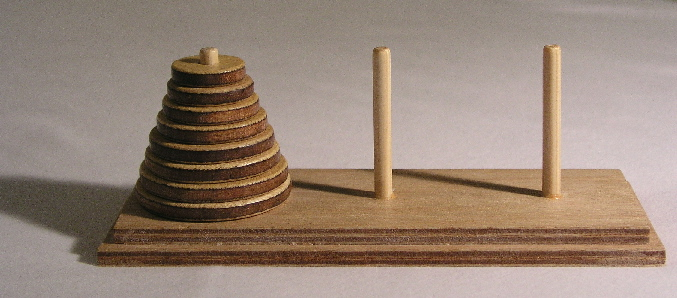
\includegraphics[width=0.8\textwidth]{img/hanoi.jpeg}
\end{figure}
\end{frame}

\begin{frame}{Exercise: Tower of Hanoi}
\begin{itemize}
\item We would like to program an algorithm that would \textit{solves} the tower of hanoi
\item Given a stack of $n$ disk to begin with, derive a program that will teach you how should you move the disks to solve the puzzle
\item Let's try to play around with the game to gain some insights and familiarity
\item Here is a link to the game: \href{https://www.mathsisfun.com/games/towerofhanoi.html}{https://www.mathsisfun.com/games/towerofhanoi.html}
\end{itemize}
\end{frame}

\begin{frame}{Solution: Tower of Hanoi}
\begin{exampleblock}{Observations:}
Suppose there are $n$ disks and suppose we know how to move $n-1$ disks from rod 1 to rod 2. Then to move $n$ disks, we just need to:
\begin{enumerate}
  \item Move all $n-1$ disk above to the rod in the middle rod
  \item Place the bottom disk to the final rod
  \item Move the $n-1$ disks to the final rod 
\end{enumerate}
\end{exampleblock}
\end{frame}

\begin{frame}{Solution: Tower of Hanoi}
\begin{itemize}
\item In other words, once we know how to move $n-1$ disks, moving $n$ disks is easy
\item But how do we know how to move $n-1$ disks?
\item Well, to move $n-1$ disk, we just need to know how to move $n-2$ disks!
\item Wait how about $n-2$? We don't know how to do that right?
\item Well, we just have to figure out how to move $n-3$ disks!
\item $\cdots$
\item But how to move $2$ disks?
\item Well, to move $2$ disks, we just need to know how to move $1$ disk
\item \textbf{But moving 1 disk is trivial!}
\end{itemize}
\end{frame}

\begin{frame}[fragile]{Coding Time}
  \begin{itemize}
    \item Now it's your time to code
    \item To help you with the starting point, consider you need to implement the function below
\begin{lstlisting}[language=python]
  def Hanoi(n,tar,emt):
    #n is the number of pile at the rod you looking at
    #tar is the number (or name) of the rod you wish to move the n pile to
    #emt is the number (or name) of the rod that is currently empty
    ###your code start below###

  #Then we ask the user to provide the number of pile to be solved, and call the function we just implemented.
  n=int(input("Enter the number of pile: "))
  Hanoi(n,3,2)
\end{lstlisting}
  \end{itemize}
\end{frame}

\begin{frame}[fragile]{Knapsack problem}
  \begin{itemize}
    \item Now we look at another problem, assuming you are a jeweller (a person who sell jewelry) and you got a chance to sell on a large market, you only get one knapsack (backpack) to carry the jewelry to the market.
    \item Certainly you want to get as many jewelries as possible so you earn more, however the size of the backpack is limited so you cannot always put all the jewelries into the backpack.
    \item Therefore you want to plan ahead to decide which jewelry and how much you should bring. However, the calculation is so annoying you want to design a program to help you so that you don't have to do it again in the future.
  \end{itemize}
\end{frame}

\begin{frame}[fragile]{Knapsack problem, formally}
  \begin{itemize}
    \item Let's try to state the problem formally, assume there are $K$ kind of jewelries, each with total value as $v_{i}$ and number $w_{i}$, then the problem statement is
    \begin{center}
      \begin{eqnarray*}
        \text{Input:}&\enspace&W\text{ : Backpack capacity}\\
        &\enspace&\{v_{1},v_{2},...,v_{K}\}\text{ : value of each jewelry}\\
        &\enspace&\{w_{1},w_{2},...,w_{K}\}\text{ : number of each jewelry}\\
        \text{Output:}&\enspace&\{n_{1},n_{2},...,n_{K}\}\text{ : number of each type of jewelry taken}\\
        \text{Subject to:}&\enspace&w_{1}n_{1}+w_{2}n_{2}+...+w_{K}n_{K}\leq W\\
        &\enspace&v_{1}n_{1}+v_{1}n_{2}+...+v_{K}n_{K}\text{ should be as large as possible}
      \end{eqnarray*}
    \end{center}
  \end{itemize}
\end{frame}

\begin{frame}[fragile]{First Attempt}
  \begin{itemize}
    \item Let's start with a simple solution
    \item Take whatever that is the most expensive!
    \item Then we only need to sort by the price and take from the tail until we cannot fit any of them.
  \end{itemize}
\end{frame}

\begin{frame}{Does it works?}
  \begin{itemize}
    \item Consider the following case, your backpack capacity is $100$ kg
    \item You got three types of Jewelry to choose from
    \begin{enumerate}
      \item Diamond, Total price: $\$90$, weight: $90$ kg
      \item Gold, Total price: $\$70$, weight: $20$ kg
      \item Emerald, Total price: $\$50$, weight: $20$ kg
    \end{enumerate}
    \item Our solution: Take $90$ kg Diamond then take $10$ kg Gold
    \item Total price: $100+70/2=\$135$
    \item What if: Take $20$ kg Gold, $20$ kg Emerald, $40$ kg Diamond?
    \item Total Price: $70+50+90*4/9=\$160>\$135$
    \item What's wrong with our solution?
  \end{itemize}
\end{frame}

\begin{frame}{Second Attempt}
  \begin{itemize}
    \item The price is total instead of unit, the diamond does not worth so much here
    \item Modified solution: Take whatever that is the most expensive \textbf{in unit price}
    \item New approach:
    \begin{enumerate}
      \item For each Jewelry, compute $u_i=v_i/w_i$, which is their unit price
      \item Sort the list by $u_i$
      \item Take the most out of the largest whenever possible
    \end{enumerate}
  \end{itemize}
\end{frame}


% \begin{frame}[fragile]{Example}
%   \begin{figure}
%     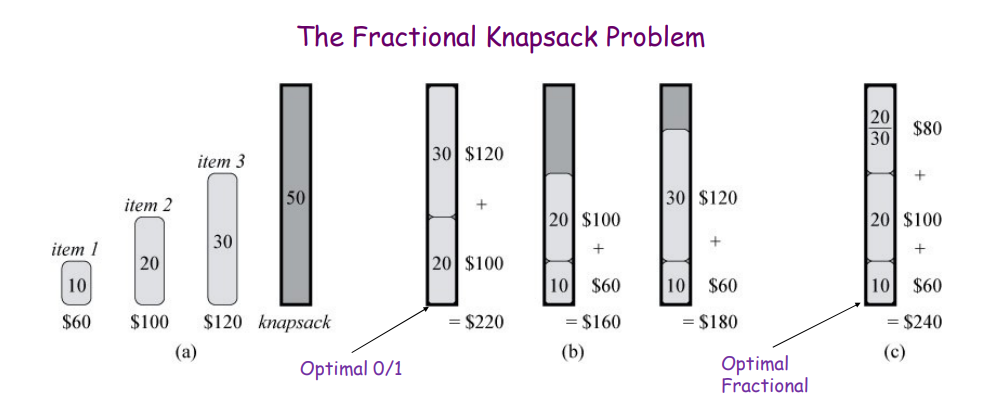
\includegraphics[width=0.8\textwidth]{img/knapsack.png}
%   \end{figure}
% \end{frame}

\begin{frame}[fragile]{Implementation}
\begin{lstlisting}[language=python]
  def Knapsack(W,v,w):
    #Treat the first two lines below as some magic, it generates a list u, each element in u is a pair with the the index and the unit price, then u is sorted in descending order
    u=[(idx,v[idx]/w[idx]) for idx in range(len(v))]
    u.sort(key=(lambda pair:pair[1]),reverse=True)
    knapsack=[]
    for jew in u:
      if w[jew[0]]<=W:
        knapsack.append((jew[0],w[jew[0]]))
        print("Take",w[jew[0]],"kg of Jewelry",jew[0])
        W=W-w[jew[0]]
      else:
        knapsack.append((jew[0],W))
        print("Take",W,"kg of Jewelry",jew[0])
        break
    return knapsack
\end{lstlisting}
\end{frame}

\begin{frame}[fragile]{Let's Try it}
  \begin{itemize}
    \item Let's try to run the code
    \item We use the same example demonstrated above, we do the following
\begin{lstlisting}[language=python]
  W=100
  v=[90,70,50]
  w=[90,20,20]
  Knapsack(W,v,w)
\end{lstlisting}
    \item Can you come up with other example?
    \item Is there any situation where this solution can fail to find the best combination?
  \end{itemize}  
\end{frame}

\begin{frame}[fragile]{Variation: 0-1 Knapsack problem}
  \begin{itemize}
    \item Now consider on top of the knapsack problem setting, we have one more rule
    \item \texttt{All or Nothing}, you either take all of one item or none of them
    \item Does our previous solution still work?
    \item No! Our method may take a portion of them item in the last step.
    \item What if we fix that? Changing the loop to 
\begin{lstlisting}[language=python]
  for jew in u:
      if w[jew[0]]<=W:
        knapsack.append((jew[0],w[jew[0]]))
        print("Take",w[jew[0]],"kg of Jewelry",jew[0])
        W=W-w[jew[0]]
\end{lstlisting}
  \end{itemize}
\end{frame}

\begin{frame}{Counter Example}
  \begin{itemize}
    \item Consider the same case but with one more jewelry, with backpack capacity $100$ kg
    \begin{enumerate}
      \item Diamond, Total price: $\$90$, weight: $90$ kg --> unit price: $\$1/kg$
      \item Gold, Total price: $\$70$, weight: $20$ kg --> unit price: $\$3.5/kg$
      \item Emerald, Total price: $\$50$, weight: $20$ kg --> unit price: $\$2.5/kg$
      \item Ruby, Total price: $\$80$, weight: $80$ kg --> unit price: $\$1/kg$
    \end{enumerate}
    \item Our solution: Take $20$ kg Gold, $20$ kg Emerald
    \item Total Price: $70+50=\$120$
    \item What if: Take $20$ kg Gold, $80$ kg Ruby
    \item Total Price: $70+80=\$150>\$120$
  \end{itemize}
\end{frame}

\begin{frame}{Greedy Algorithm and its downside}
  \begin{itemize}
    \item What we have been using is called the Greedy algorithm
    \item We also take the best choice we have at each step
    \item Benefits:
    \begin{itemize}
      \item Easy to implement
      \item Intuitive to reason
      \item Efficient, the most time taken in sorting
    \end{itemize}
    \item Problem: May not always be optimal
  \end{itemize}
\end{frame}

\begin{frame}{Dynamic Programming to the rescue!}
  \begin{itemize}
    \item As in recursion, we will try to break the problem into smaller problem
    \item Consider you have the solution to $n$ items with any weight limit $W$, denote it as $OPT(n,W)$
    \item Now we add one more item into the list, what is the new solution?
    \item Observation: You either take the new item, with value $v$ and weight $w$, or you don't.
    \item Sounds obvious right? But that what we want, so now we know
    \begin{equation}
      OPT(n+1,W) = \max(OPT(n,W),OPT(n,W-w)+v)\label{DP}
    \end{equation}
    \item But wait, aren't we trying to make the problem smaller?
    \item We can start from $n=1$ and gradually increase it.
  \end{itemize}
\end{frame}

\begin{frame}{Solution}
  \begin{enumerate}
    \item Build up a table $DP$ with $n+1$ rows and $W$ column
    \item Set $DP[0][w]$ to be $0$ if $w_0<w$ and $v_0$ otherwise
    \item Loop from $k=1$ to $n$ and $w=0$ to $W$, fill in the table $DP[k][w]$ according to equation (\ref{DP})
    \item return $DP[n][W]$
  \end{enumerate}
\end{frame}

\begin{frame}[fragile]{Implementation}
\begin{lstlisting}[language=python]
  def DPKnapsack(W,v,w):
    DP=[[0]*(W+1)]
    DP[0][w[0]:]=[v[0]]*(W-w[0]+1)
    for i in range(1,len(v)):
      DP.append([0]*(W+1))
      for j in range(W+1):
        if j<w[i]:
          DP[i][j] = DP[i-1][j]
        else:
          DP[i][j] = max(DP[i-1][j],DP[i-1][j-w[i]]+v[i])
    return DP[len(v)-1][W]
\end{lstlisting}
\end{frame}

\begin{frame}{Exercise}
  \begin{itemize}
    \item Let's try to test the code against our previous counter example and see what is the result
    \item Challenge: Modify the above code so that we also know which jewelries are taken
  \end{itemize}
\end{frame}
% \begin{frame}[fragile]{First problem!}
%   \begin{itemize}
%     \item Suppose now you work as a cashier, you job is to collect bills from customer and make changes
%     \item The shop is small and the things are cheap so most of the customers are paying by coin, but still there are some customers pay by notes.
%     \item So when customers pay be notes, you need to make changes, let's say you have a bunch (much more than the amount u need to change) of coin, which are of value $1$, $2$ and $5$ respectively.
%     \item Clearly no one like to receive a bunch of coin in change, so in order not to piss off anyone you need to find a way to minimize the number of coin used for changes.
%   \end{itemize}
% \end{frame}

% \begin{frame}[fragile]{Problem statement}
%   \begin{itemize}
%     \item Now clearly you have a problem to solve, but it is complicated and contain a lot of unnecessary information, we need to simplify it.
%     \item Recall the framework of program that we emphasize in previous lectures, a program is usually in the form of
%     \begin{itemize}
%       \item input
%       \item process
%       \item output
%     \end{itemize}
%     \item But as a user to use the program you designed, they don't really care what is the process happened behind the code, all they care is if the output correctly answer their input!
%     \item So we need to first make it clear what are the input and expected output of the problem, then work out the process between
%   \end{itemize}
% \end{frame}

% \begin{frame}[fragile]{Change making problem}
%   \begin{center}
%     \begin{eqnarray*}
%       \text{Input:}&\enspace&\$C\text{ :changes to be made}\\
%       \text{Output:}&\enspace&\{n_{1},n_{2},n_{5}\}\text{ : number of each type of coins used}\\
%       \text{Subject to:}&\enspace&n_{1}+2n_{2}+5n_{5}=C\\
%       &\enspace&n_{1}+n_{2}+n_{5}\text{ should be as small as possible}
%     \end{eqnarray*}
%   \end{center}
% \end{frame}

% \begin{frame}[fragile]{First Attempt}
%   \begin{itemize}
%     \item Now let's think about how to solve the problem
%     \item our main target is to give as less coin as possible
%     \item what would be the easiest way to do so?
%   \end{itemize}
% \end{frame}

% \begin{frame}[fragile]{First Attempt}
%   \begin{itemize}
%     \item Now let's think about how to solve the problem
%     \item our main target is to give as less coin as possible
%     \item what would be the easiest way to do so?
%     \item Perhaps always use the largest coin possible?
%   \end{itemize}
% \end{frame}

% \begin{frame}[fragile]{Example}
%   \begin{itemize}
%     \item Let's try it on a actual example!
%     \item Let's say the change we need to make is \$$9$
%     \item Then we first use the largest coin, which is \$$5$, then we still need to change for \$$4$
%     \item Next since $4<5$, we cannot use \$$5$ coin, so our choice will be \$$2$, then we are remained with \$$2$
%     \item Finally the result is trivial that we shall use one more \$$2$ coin to change
%     \item So our solution would be $\{0,2,1\}$, which stands for we use $0$ \$$1$ coin, $2$ \$$2$ coin and $1$ \$$5$ coin.
%     \item But is it optimal?
%   \end{itemize}
% \end{frame}

% \begin{frame}[fragile]{Example cont'd}
%   \begin{itemize}
%     \item Yes! But how can we prove it?
%     \item For this case we used three coins, obviously we cannot make the changes using one coin only since there is no \$ $9$ coin, but what about two?
%     \item $1+1=2$,$2+2=4$,$5+5=10$,$1+2=3$,$1+5=6$,$2+5=7$
%     \item None of the combinations equal to $9$!
%     \item So it is also impossible to make the changes using only two coins
%     \item Therefore three is optimal!
%   \end{itemize}
% \end{frame}

% \begin{frame}[fragile]{Implementation}
%   \begin{itemize}
%     \item So now we have an idea, let's try to implement it!
% \begin{lstlisting}[language=python]
%   price=int(input("Enter the bill:"))
%   payment=int(input("Enter the payment:"))
%   while payment<price:  #check whether customer pay enough money
%     print("payment not enough, please pay again")
%     payment=int(input("Enter the payment:"))
%   C=payment-price
%   n5=C//5   #here we use C//5 instead of C-5
%   C=C%5
%   n2=C//2
%   C=C%2
%   n1=C
%   print("change:",n1,"$1 coin,"n2,"$2 coin",n5,"$5 coin")
% \end{lstlisting}
%   \end{itemize}
% \end{frame}

% \begin{frame}[fragile]{Improvement}
%   \begin{itemize}
%     \item In the program, we assumed the coin we have is always fixed, i.e. \$$1$,\$$2$ and \$$5$
%     \item let's make it more flexible (so that perhaps it can be used in other countries' store)
%     \item To do some we need to borrow the power of math
%     \item let's $K$ be the number of distinct value of coin we have
%     \item then let's $c_{1},c_{2},...,c_{K}$ be the value of each of the coin
%     \item for simplicity we assume the coin is given in ascending order, i.e.
%     $$c_{1}>c_{2}>...>c_{K}$$
%     \item also we always assume $c_{K}=1$, so that any change can be made
%   \end{itemize}
% \end{frame}

% \begin{frame}[fragile]{New problem statement}
%   \begin{itemize}
%     \item Then we can rewrite our problem as
%     \begin{center}
%       \begin{eqnarray*}
%         \text{Input:}&\enspace&C\text{ : changes to be made}\\
%         &\enspace&\{c_{1},c_{2},...,c_{K}\}\text{ : value of each coin}\\
%         \text{Output:}&\enspace&\{n_{1},n_{2},...,n_{K}\}\text{ : number of each type of coins used}\\
%         \text{Subject to:}&\enspace&c_{1}n_{1}+c_{2}n_{2}+...+c_{K}n_{K}=C\\
%         &\enspace&n_{1}+n_{2}+...+n_{K}\text{ should be as small as possible}
%       \end{eqnarray*}
%     \end{center}
%   \end{itemize}
% \end{frame}

% \begin{frame}[fragile]{New Implementation}
%   \begin{itemize}
%     \item Then we update the implementation
% \begin{lstlisting}[language=python]
%   #we skipped the part of getting payment, price and C.
%   N=int(input("Input number of types of coin:"))
%   coins=[]
%   for i in range(N):
%     coins.append(int(input("Input the coin value:")))
%   coins.sort(reverse=True)
%   n=[];
%   for i in range(N):
%     n.append(C//coins[i])
%     C=C%coins[i]
%   print("change:",n)
% \end{lstlisting}
%   \end{itemize}
% \end{frame}

% \begin{frame}[fragile]{Greedy Algorithm}
%   \begin{itemize}
%     \item What we just did is a kind of approach call Greedy Algorithm
%     \item As the name \textbf{Greedy} suggest, it means the program always make the best choice it can made at each step and construct the solution
%     \item Advantage:
%     \begin{itemize}
%       \item Simple to understand
%       \item Easy to implement
%       \item Efficient
%     \end{itemize}
%     \item Application: Minimum spanning tree, Travelling salesman problem...
%     \item But what about the disadvantage?
%   \end{itemize}
% \end{frame}

% \begin{frame}[fragile]{Further example}
%   \begin{itemize}
%     \item Let's consider the same problem, but this time we have different coins
%     \item we have \$$1$, \$$10$ and \$$25$
%     \item Then let's say this time we need to give a change of \$$30$
%     \item What will our program give?
%   \end{itemize}
% \end{frame}

% \begin{frame}[fragile]{Further example}
%   \begin{itemize}
%     \item Let's consider the same problem, but this time we have different coins
%     \item we have \$$1$, \$$10$ and \$$25$
%     \item Then let's say this time we need to give a change of \$$30$
%     \item What will our program give?
%     \item Since we are always taking the largest possible coin, it will gives $5\times \$1$ and $1\times \$25$, which is $6$ coin in total
%     \item Is this optimal?
%   \end{itemize}
% \end{frame}

% \begin{frame}[fragile]{Further example}
%   \begin{itemize}
%     \item Let's consider the same problem, but this time we have different coins
%     \item we have \$$1$, \$$10$ and \$$25$
%     \item Then let's say this time we need to give a change of \$$30$
%     \item What will our program give?
%     \item Since we are always taking the largest possible coin, it will gives $5\times \$1$ and $1\times \$25$, which is $6$ coins in total
%     \item Is this optimal?
%     \item No! We can simply give $3\times \$10$ which gives only $3$ coins!
%   \end{itemize}
% \end{frame}

% \begin{frame}[fragile]{Problem of Greedy Algorithm}
%   \begin{itemize}
%     \item Since we only consider the best solution we can obtain at each step of our program
%     \item It might not be the best choice for the overall problem
%     \item Greedy algorithm may not lways give the best answer
%     \item Does that means Greedy algorithm is useless?
%   \end{itemize}
% \end{frame}

% \begin{frame}[fragile]{Problem of Greedy Algorithm}
%   \begin{itemize}
%     \item Since we only consider the best solution we can obtain at each step of our program
%     \item It might not be the best choice for the overall problem
%     \item Greedy algorithm may not lways give the best answer
%     \item Does that means Greedy algorithm is useless?
%     \item No, we still use Greedy algorithm in practice, there are two cases we will use it
%     \begin{enumerate}
%       \item The greedy algorithm can be proven to be optimal
%       \item We accept approximated solution (not optimal, but not too far from it)
%     \end{enumerate}
%   \end{itemize}
% \end{frame}

\end{document}
